\section{Diskussion}
\label{sec:Diskussion}
Die Messwerte weisen eine große Abweichung im Vergleich zu den Theoriewerten auf.  \\
Trotzdessen, dass $(4,46 \pm 0,18) \cdot 10^{-3} \,\,\unit{\kilo\gram\meter\squared}$ keinen Theoriewert hat, kann angenommen werden, dass 
dieser Wert ungenau ist, da der Stab 
als masselos angenommen wird. Dies verfälscht $I_{\text{Drill}}$ signifikant. Die Winkelrichtgröße 
$D = (21,0 \pm 0,8) \cdot 10^{-3} \,\,\unit{\newton\meter}$ kann auch als eine Größe mit großer Messunsicherheit angenommen
werden, da es nicht möglich war gleichzeitig den Auslenkungswinkel und die benötigte Kraft exakt zu bestimmen. Es könnte zu einem großen 
Fehler durch Messparalaxe gekommen sein, der je nach Betrachtungswinkel unterschiedlich groß wäre. Durch diesen Umstand sind auch sämtliche 
Größen, die von $D$ abgeleitet wurden, mit großen Fehlern behaftet. \\
Aufgrund der existierenden Reibung während des Versuchs, werden die 
Periodendauern kleiner als sie eigentlich ohne Reibung wären. Dies könnte erklären, warum die gemessenen Werte durchgehend kleiner sind als die 
Theoriewerte. Außerdem kommt durch die Reaktionszeit der messenden Person eine weitere Ungenauigkeit hinzu, die sämtliche gemessenen 
Trägheitsmomente betrifft.\\
Das Trägheitsmoment der Scheibe $(1,85 \pm 0,07) \cdot 10^{-3} \,\,\unit{\kilo\gram\meter\squared}$ hat eine Abweichung von $37,95 \,\,\%$ 
zum Theoriewert $(2,552 \pm 0,006) \cdot 10^{-3} \,\,\unit{\kilo\gram\meter\squared}$.\\
Das Trägheitsmoment der Kugel $(1,90 \pm 0,08) \cdot 10^{-3} \,\,\unit{\kilo\gram\meter\squared}$ hat eine prozentuale 
Abweichung von $32,84 \,\,\%$ zum Theoriewert $(2,524 \pm 0,007) \cdot 10^{-3} \,\,\unit{\kilo\gram\meter\squared}$. \\
Als zusätzliche Fehlerquelle kommt bei der Berechnung des Trägheitsmoments der Puppe hinzu, dass die Periodendauer so klein war, dass selbst eine
Messung von $5\,T$ ungenau war. Das Trägheitsmoment der Puppe in Position 1 beträgt $(0,2 \pm 0,008) \cdot 10^{-3}\,\, \unit{\kilo\gram\meter\squared}$.
 Die Abweichung ist $31,00 \,\,\%$ zum Theoriewert von $(0,262 \pm 0,025) \cdot 10^{-3}\,\, \unit{\kilo\gram\meter\squared}$.\\
Das Trägheitsmoment der Puppe in Position 2 ist $ (0,491 \pm 0,020) \cdot 10^{-3}\,\, \unit{\kilo\gram\meter\squared}$ und die Abweichung beträgt 46,64 \,\,\% zum Theoriewert 
von $(0,72 \pm 0,05) \cdot 10^{-3}\,\, \unit{\kilo\gram\meter\squared}$.\\
Das Verhältnis vom Trägheitsmoment der Puppe in Position 1 zu dem in Position 2 ist $\frac{I_{\text{Pos1}}}{I_{\text{Pos2}}} = 0,4073$. Das
Verhältnis der Theorieträgheitsmomente ist $\frac{I_{\text{Pos1,theo}}}{I_{\text{Pos2,theo}}} = 0,3639$. Die Abweichung des gemessenen Verhältnis im
Vergleich zum theoretischen Verhältnis beträgt $10,66 \,\,\%$. Diese Abweichung ist deutlich geringer als die Abweichung der einzelnen Trägheitsmomente 
zum Theoriewert. 
 
\section{Originaldaten}
\label{sec:Originaldaten}
% \begin{figure}[H]
%   \centering
%   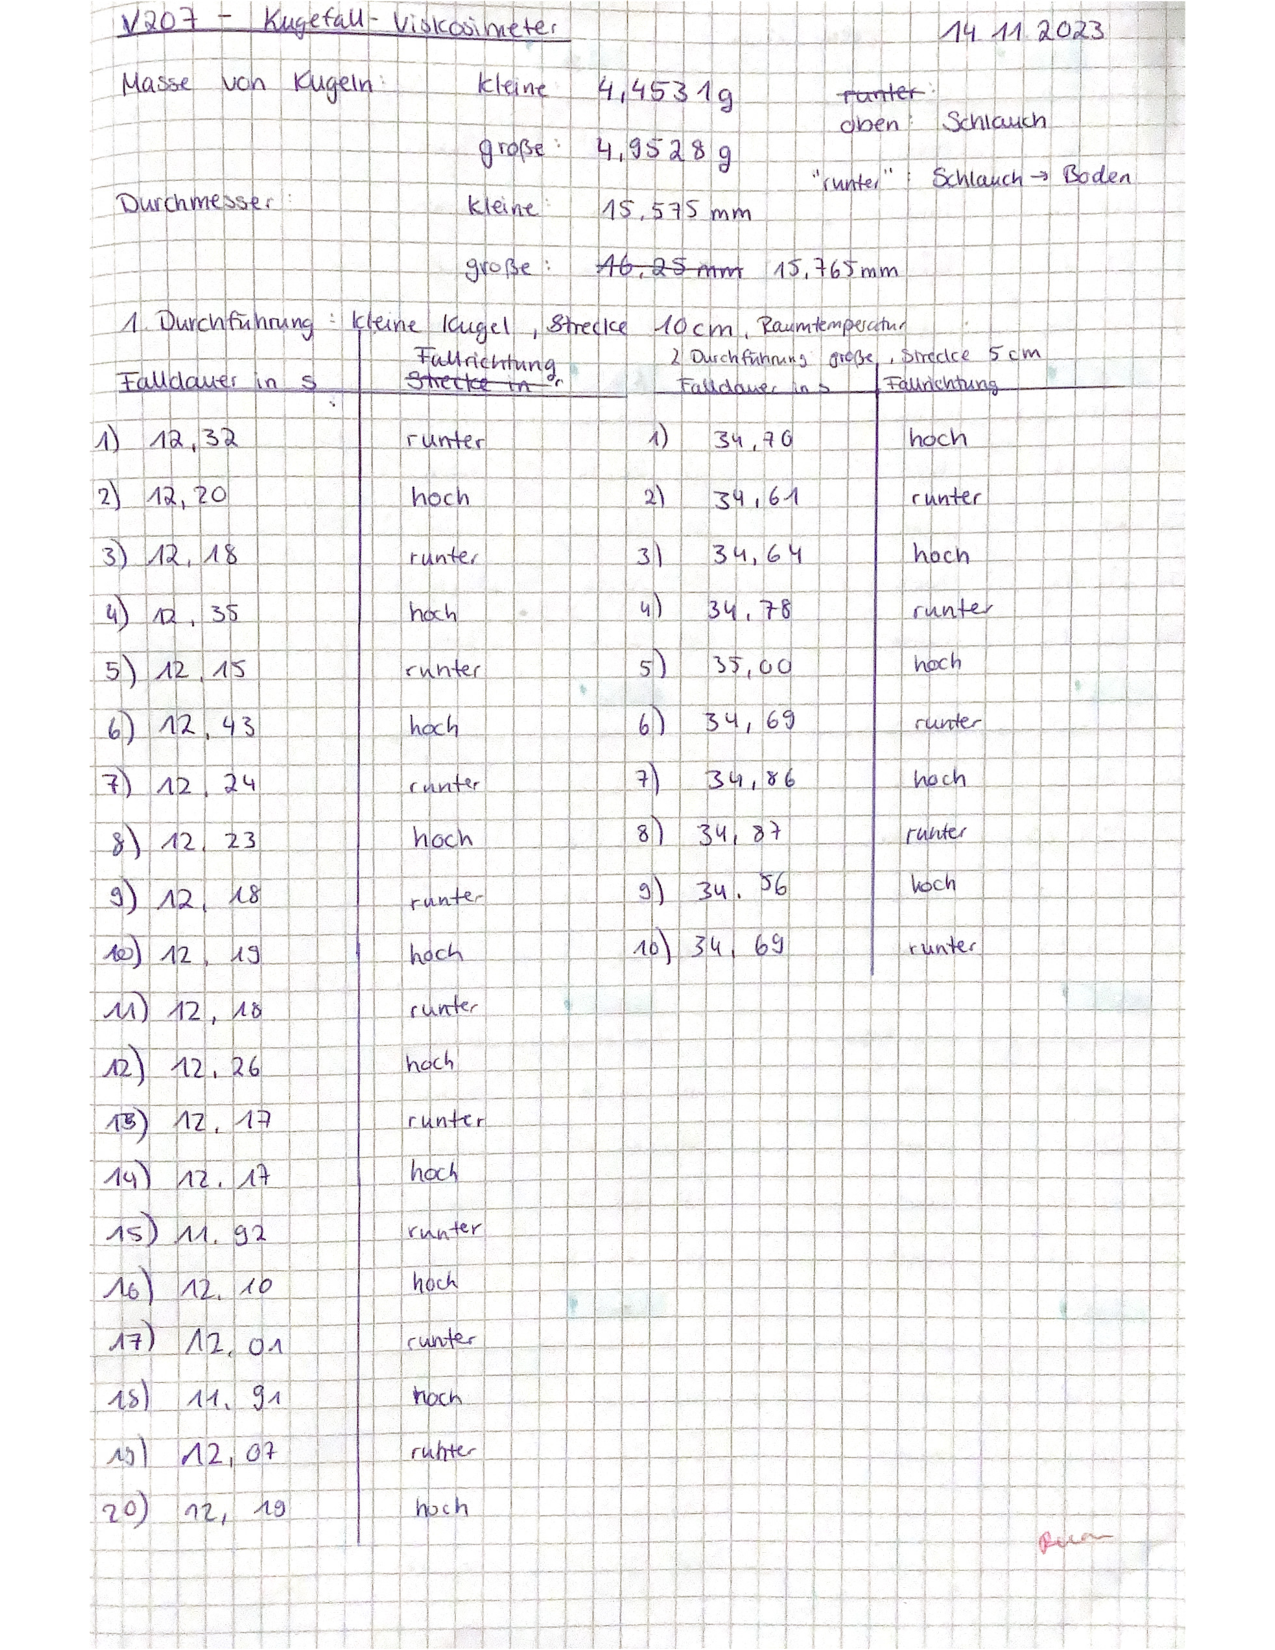
\includegraphics[width=\textwidth]{Messwerte.pdf}
%   \label{fig:Messungen}
% \end{figure}